%$$$$$$$$$$$$$$$$$$$$$$$$$$$$$$$$$$$$$$$$$$$$$$$$$$$$$$$$$$$$$$$$$$$$$$$$$$$$$$$$$$$
%----------------------------------------------------------------------Introducci�n-
\section{Metodolog�a Propuesta}
%$$$$$$$$$$$$$$$$$$$$$$$$$$$$$$$$$$$$$$$$$$$$$$$$$$$$$$$$$$$$$$$$$$$$$$$$$$$$$$$$$$$


\begin{frame}
\frametitle{Metodolog�a Propuesta} 

\begin{figure}
\begin{tikzpicture}[node distance=0.5cm, auto,>=latex', thick]
\scriptsize
    % We need to set at bounding box first. Otherwise the diagram
    % will change position for each frame.
    \path[use as bounding box] (-1.5,0) rectangle (12,-2);

    % TT methodology     
    \node [phase]                        (monitoreo)     {Vigilancia};
    \node [phase, below of=monitoreo]    (choice)        {Elecci�n};
    \node [phase, below of=choice]       (acquisition)   {Adquisici�n};
    \node [phase, below of=acquisition]  (adaptation)    {Adaptaci�n};
    \node [phase, below of=adaptation]   (absortion)     {Absorci�n};
    \node [phase, below of=absortion]    (aplication)    {Aplicaci�n};
    \node [phase, below of=aplication]   (difusion)      {Difusi�n};

    % linuxencaja + investigaci�n
    \path (difusion.south) +(0,-0.2) node (research)     {Investigaci�n Universitaria};
    \path (monitoreo.north)+(0,+0.2) node (linuxencaja)  {Comunidad \textit{linuxencaja}};

    % Now it's time to draw the colored rectangles.
     \begin{pgfonlayer}{background}
        \path (linuxencaja.west |- linuxencaja.north) + (-0.2,0.0)  node (a) {};
        \path (research.south   -| research.east)     + (+0.1,-0.15) node (b) {};
        \path (research.east    |- research.east)     + (+0.1,-0.1) node (c) {};
        \path[fill=yellow!20,rounded corners, draw=black!50] (a) rectangle (c);           
        \path (monitoreo.north west)+(-0.2,0.2) node (a) {};
    \end{pgfonlayer}

    % "Empresa" node
    \node [industry, right=1cm of linuxencaja.north east]  (industry)      {\textcolor{Lavender} {. \\ . \\.} \textbf{ \large Empresa} \textcolor{Lavender} {. \\ . \\.}
%                                                                   \begin{itemize}
%                                                                    \item Transferencia de conocimiento.
%                                                                      \begin{itemize}
%                                                                        \scriptsize
%                                                                        \item Procesos de fabricaci�n.
%                                                                        \item Metodolog�as de dise�o.
%                                                                      \end{itemize}
%                                                                    \item Dise�os de referencia.
%                                                                   \end{itemize} 
                                                                   };

    \draw[myarrow2] ([xshift=0.75cm] adaptation.east) -- ++(0.2,0)-- ++ (0,2.2) --  (industry.west);	

    % "Academia" node
    \node [academy, right=0.8cm of research.south east]  (academy)      {\textcolor{Lavender} {.\\ . \\.}\textbf{ \large Academia} \textcolor{Lavender} {.\\ . \\.}
%                                                                   \begin{itemize}
%                                                                    \item Actualizaci�n de programas acad�micos.
%                                                                    \item Generaci�n de habilidades.
%                                                                    \item Creaci�n de industria.
%                                                                    \item Creaci�n/adaptaci�n de metodolog�as /procesos de dise�o.
%                                                                   \end{itemize}  
                                                                      };
    \draw[myarrow1] ([xshift=0.75cm] adaptation.east) -- ++(0.2,0)-- ++ (0,-2.2) --  (academy.west);	


    % Relaciones Universidad - Empresa    
    \draw[myarrow] ([xshift=-2.6cm] industry.south) -- ([xshift=-2.6cm] academy.north);
%     \node[mylabel, below left=of industry.south] (label1)  {\scriptsize Pasant�as.\\Servicios.\\Regal�as.    \\Necesidades.};  

    % Relaciones Empresa - Universidad
    \draw[myarrow] ([xshift= 2.6cm] academy.north)  -- ([xshift= 2.6cm] industry.south);
%     \node[mylabel, below right=of industry.south] (label1) {\scriptsize Creaci�n. \\Soporte.  \\Capacitaci�n.\\Personal.};  

    % Necesidades de la sociedad
    \node [extern, right=0.2cm of industry] (needs)   {Necesidades de la sociedad};
    \draw[myarrow] (needs.west)  --  (industry.east);
    \draw[myarrow] (needs.south) -- ++(0, -3.85) -- (academy.east);

    % Realimentaci�n Universidad - Empresa a la metodolog�a de transferencia
    \draw[myarrow] (industry.north)  --++(0,0.3)--++(-5.65,0) -- ([yshift= 0cm] linuxencaja.north);
    \draw[myarrow] (academy.south)  --++(0,-0.3)--++(-5.65,0) -- ([yshift= 0.1cm] research.south);
    \node[mylabel2, above left=of industry.north] (label1) {\scriptsize Necesidades, Personal, Conocimientos};  
    \node[mylabel2, below left=of academy.south]  (label2) {\scriptsize Necesidades, Personal, Conocimientos}; 
\end{tikzpicture}
\end{figure}

\end{frame}


% \begin{frame}
%   \begin{center} 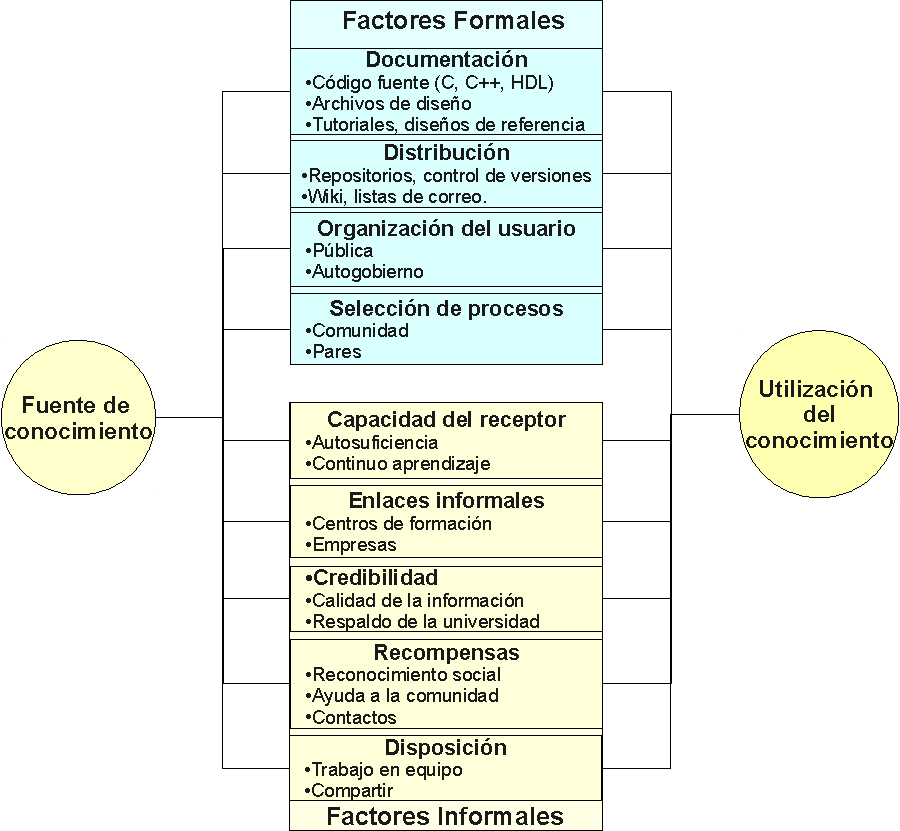
\includegraphics[scale=.6]{../images/transfer_model.pdf}   \end{center}
% \end{frame}





